% set documentclass - this will make the file compile if open in editor
\documentclass[a4paper,12pt,fullpage,openany,hyperfootnotes,hidelinks]{scrbook}

% load Tikz & related packages
\usepackage{tikz}
\usetikzlibrary{matrix,arrows.meta,fit,positioning,shapes,automata}

% document must begin
\begin{document}

% notes on graphics goal / textual description of what is to be conveyed

demonstrate in a very simple way the 4 layers of swarm, as described in : 

conceive of Swarm as having clearly separable layers (see figure ), each dependent on the previous one: (1) a peer-to-peer network protocol to serve as underlay transport, (2) an overlay network with protocols powering a distributed immutable storage of chunk (fix-sized data blocks), (3) a component for higher-level data access defining APIs for the base-layer features, and (4) an application layer potentially defining the standards, capturing best practices for more elaborate use-cases. We regard (2) and (3) as the core of Swarm.


% existing sketch of the graphics
% INSERT
\begin{figure}[htp]
    \centering
    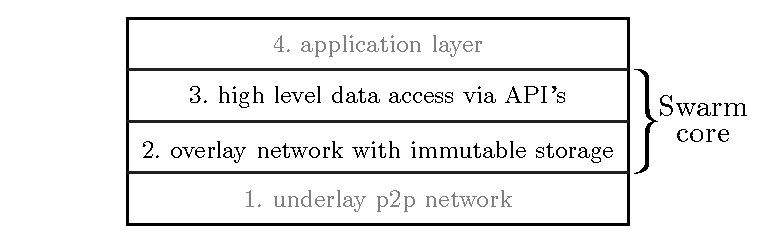
\includegraphics[width=10cm]{fig-drafts/swarm-layered-design.pdf}
\end{figure}

% simple example Tikz "picture"
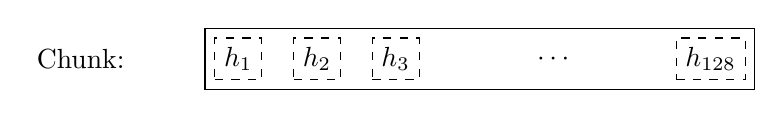
\begin{tikzpicture}
\node at (0,1) {Chunk:};
\node[draw,dashed] (h1) at (2,1) {$h_1$};
\node[draw,dashed] (h2) at (3,1) {$h_2$};
\node[draw,dashed] (h3) at (4,1) {$h_3$};
\node (dots) at (6,1) {$\cdots$};
\node[draw,dashed] (h128) at (8,1) {$h_{128}$};
\node[draw,fit=(h1) (h2) (h3) (dots) (h128)]{};
\end{tikzpicture}

% document must end
\end{document}